\documentclass[a4paper, 14pt]{extarticle}

% Поля
%--------------------------------------
\usepackage{geometry}
\geometry{a4paper,tmargin=2cm,bmargin=2cm,lmargin=3cm,rmargin=1cm}
%--------------------------------------


%Russian-specific packages
%--------------------------------------
\usepackage[T2A]{fontenc}
\usepackage[utf8]{inputenc}
\usepackage[english, main=russian]{babel}

%--------------------------------------

\usepackage{textcomp}

% Красная строка
%--------------------------------------
\usepackage{indentfirst}               
%--------------------------------------             


%Graphics
%--------------------------------------
\usepackage{graphicx}
\graphicspath{ {../images/} {./images/} }
\usepackage{float}%"Плавающие" картинки
%--------------------------------------

% Полуторный интервал
%--------------------------------------
\linespread{1.3}                    
%--------------------------------------

% Уменьшение расстояний между плавающими объектами
%--------------------------------------
\setlength{\floatsep}{10pt plus 2pt minus 2pt}
\setlength{\textfloatsep}{15pt plus 2pt minus 4pt}
\setlength{\intextsep}{10pt plus 2pt minus 2pt}
%--------------------------------------

%Выравнивание и переносы
%--------------------------------------
% Избавляемся от переполнений
\sloppy
% Запрещаем разрыв страницы после первой строки абзаца
\clubpenalty=10000
% Запрещаем разрыв страницы после последней строки абзаца
\widowpenalty=10000
%--------------------------------------

%Списки
\usepackage{enumitem}

\usepackage{minted}
%Подписи
\usepackage{caption} 

%Гиперссылки
% \usepackage{hyperref}

\usepackage[colorlinks, urlcolor = blue, filecolor = blue, citecolor = blue, linkcolor = black]{hyperref}


\hypersetup {
unicode=true
}

%Рисунки
%--------------------------------------
\DeclareCaptionLabelSeparator*{emdash}{~--- }
\captionsetup[figure]{labelsep=emdash,font=onehalfspacing,position=bottom}
%--------------------------------------

\usepackage{tempora}

%Листинги
%--------------------------------------
%Листинги
%--------------------------------------
\usepackage{listings}
\lstset{
  basicstyle=\ttfamily\footnotesize, 
  %basicstyle=\footnotesize\AnkaCoder,        % the size of the fonts that are used for the code
  breakatwhitespace=false,         % sets if automatic breaks shoulbd only happen at whitespace
  breaklines=true,                 % sets automatic line breaking
  captionpos=t,                    % sets the caption-position to bottom
  inputencoding=utf8,
  frame=single,                    % adds a frame around the code
  keepspaces=true,                 % keeps spaces in text, useful for keeping indentation of code (possibly needs columns=flexible)
  keywordstyle=\bf,       % keyword style
  numbers=left,                    % where to put the line-numbers; possible values are (none, left, right)
  numbersep=5pt,                   % how far the line-numbers are from the code
  xleftmargin=25pt,
  xrightmargin=25pt,
  showspaces=false,                % show spaces everywhere adding particular underscores; it overrides 'showstringspaces'
  showstringspaces=false,          % underline spaces within strings only
  showtabs=false,                  % show tabs within strings adding particular underscores
  stepnumber=1,                    % the step between two line-numbers. If it's 1, each line will be numbered
  tabsize=2,                       % sets default tabsize to 8 spaces
  title=\lstname                   % show the filename of files included with \lstinputlisting; also try caption instead of title
}
%--------------------------------------

%%% Математические пакеты %%%
%--------------------------------------
\usepackage{amsthm,amsfonts,amsmath,amssymb,amscd}  % Математические дополнения от AMS
\usepackage{mathtools}                              % Добавляет окружение multlined
\usepackage[perpage]{footmisc}


% графики
\usepackage{booktabs}        % Пакет для улучшенных таблиц
\usepackage{pgfplots}        % Пакет для построения графиков
\pgfplotsset{compat=1.17}    % Установка совместимости
\usepackage{tikz}            % Пакет для создания схем
\usetikzlibrary{positioning, arrows.meta}  % Библиотеки для TikZ
\usepackage{placeins}        % \FloatBarrier (фиксируем плавающие объекты по разделам)

% Литература 

% переименовываем  список литературы в "список используемой литературы"
\addto\captionsrussian{\def\refname{Список литературы}}



\captionsetup[figure]{name=Рисунок, labelsep=space}


%--------------------------------------

%--------------------------------------
%			НАЧАЛО ДОКУМЕНТА
%--------------------------------------

\begin{document}

%--------------------------------------
%			ТИТУЛЬНЫЙ ЛИСТ
%--------------------------------------
\begin{titlepage}
\thispagestyle{empty}
\newpage


%Шапка титульного листа
%--------------------------------------
\vspace*{-60pt}
\hspace{-65pt}
\begin{minipage}{0.3\textwidth}
\hspace*{-20pt}\centering
\includegraphics[width=\textwidth]{emblem}
\end{minipage}
\begin{minipage}{0.67\textwidth}\small \textbf{
\vspace*{-0.7ex}
\hspace*{-6pt}\centerline{Министерство науки и высшего образования Российской Федерации}
\vspace*{-0.7ex}
\centerline{Федеральное государственное автономное образовательное учреждение }
\vspace*{-0.7ex}
\centerline{высшего образования}
\vspace*{-0.7ex}
\centerline{<<Московский государственный технический университет}
\vspace*{-0.7ex}
\centerline{имени Н.Э. Баумана}
\vspace*{-0.7ex}
\centerline{(национальный исследовательский университет)>>}
\vspace*{-0.7ex}
\centerline{(МГТУ им. Н.Э. Баумана)}}
\end{minipage}
%--------------------------------------

%Полосы
%--------------------------------------
\vspace{-25pt}
\hspace{-35pt}\rule{\textwidth}{2.3pt}

\vspace*{-20.3pt}
\hspace{-35pt}\rule{\textwidth}{0.4pt}
%--------------------------------------

\vspace{1.5ex}
\hspace{-35pt} \noindent \small ФАКУЛЬТЕТ\hspace{80pt} <<Информатика и системы управления>>

\vspace*{-16pt}
\hspace{47pt}\rule{0.83\textwidth}{0.4pt}

\vspace{0.5ex}
\hspace{-35pt} \noindent \small КАФЕДРА\hspace{50pt} <<Теоретическая информатика и компьютерные технологии>>

\vspace*{-16pt}
\hspace{30pt}\rule{0.866\textwidth}{0.4pt}

\vspace{11em}

\begin{center}
\Large {\bf Лабораторная работа №4} \\ 
\large <<Построение предсказательной модели>> \\
\large {по курсу <<Моделирование>>} \\

\end{center}\normalsize

\vspace{8em}

\vbox{%
\hfill%
\vbox{%
\hbox{Студент: Аринин М.А.}%
\hbox{Группа: ИУ9-82Б}%
\hbox{Преподаватель: Домрачева А.Б.}%
}%
} 

\bigskip

\vfill


\begin{center}
\textsl{Москва 2026}
\end{center}
\end{titlepage}
%--------------------------------------
%		КОНЕЦ ТИТУЛЬНОГО ЛИСТА
%--------------------------------------


\renewcommand{\ttdefault}{pcr}

\setlength{\tabcolsep}{3pt}

\newpage
\setcounter{page}{2}

%--------------------------------------------------------------------
\section{Постановка задачи}

Имеется датасет \texttt{diabetes.csv} из 768 наблюдений. В качестве зависимой переменной выбрана
\texttt{Glucose} (уровень глюкозы). Контрольный признак \texttt{Outcome} не используется при построении модели.
По условию также исключается признак \texttt{Insulin}. Таким образом, после исключений остаются 6 факторов:
\[
\begin{multlined}
X = (\texttt{Pregnancies},\ \texttt{BloodPressure},\ \texttt{SkinThickness},\ \texttt{BMI},\\
\texttt{DiabetesPedigreeFunction},\ \texttt{Age}).
\end{multlined}
\]

Цель работы --- построить статистическую вычислительную модель, позволяющую по значениям факторов
оценивать уровень глюкозы, а также (при необходимости) сократить число факторов, обосновав выбор.

\textbf{Входные данные:}
\begin{itemize}
  \item файл \texttt{diabetes.csv} (\texttt{https://disk.yandex.ru/i/M35XVBrxn09\_iQ});
  \item $Y=\texttt{Glucose}$;
  \item $X$ --- перечисленные 6 признаков.
\end{itemize}

\textbf{Описание признаков (семантика столбцов).}
\begin{enumerate}
  \item \texttt{Pregnancies} --- количество беременностей (ед.).
  \item \texttt{Glucose} --- результат двухчасового перорального теста на толерантность к глюкозе (мг/дл).
  \item \texttt{BloodPressure} --- диастолическое артериальное давление (мм рт.\,ст.).
  \item \texttt{SkinThickness} --- толщина кожной складки трицепса (мм).
  \item \texttt{Insulin} --- результат двухчасового теста на содержание инсулина в сыворотке крови (мкЕд/мл).
  \item \texttt{BMI} --- индекс массы тела: вес (кг) / рост$^2$ (м$^2$).
  \item \texttt{DiabetesPedigreeFunction} --- показатель наследственной предрасположенности (безразмерный).
  \item \texttt{Age} --- возраст пациента (полных лет).
  \item \texttt{Outcome} --- 1, если пациент отправлен на дополнительное обследование.
\end{enumerate}

\textbf{Выходные данные:}
\begin{itemize}
  \item выбранный набор факторов (оптимальная размерность $p$);
  \item оценённые параметры модели;
  \item результаты проверок гипотез и качества модели.
\end{itemize}

%--------------------------------------------------------------------
\section{Построение математической модели}

\textbf{Тип модели.} Задача относится к методам многомерного статистического анализа. Рассматривается стохастическая статистическая модель, поскольку входные данные представлены выборкой наблюдений (случайных величин/векторов), а искомая зависимость устанавливается по статистическим оценкам и проверкам гипотез. В терминах предсказательных моделей это означает, что строится отображение ``объект $\to$ ответ'', а параметры выбираются по данным; при этом в регрессионной постановке учитывается случайная ошибка (шум) $\varepsilon$.

\subsection{Формализация задачи в общем виде}
Пусть задана выборка из $n$ наблюдений $(x^{(k)},y^{(k)})$, где $y^{(k)}\in\mathbb{R}$ --- значение зависимой
переменной (уровень глюкозы), а $x^{(k)}\in\mathbb{R}^{p}$ --- вектор факторов. Требуется построить модель вида
\[
\hat{y} = f(x;\,\theta),
\]
где $\theta$ --- вектор неизвестных параметров, оцененных по выборке.

\medskip
\textbf{Общий вид предсказательной модели.} В общем виде предсказательная модель задаётся отображением
\[
a: X\times W \to Y,
\]
где $X$ --- множество объектов (векторов признаков), $W$ --- множество параметров модели, $Y$ --- множество ответов.
Так как ответ $Y$ является вещественным числом (\texttt{Glucose}), задача относится к \textit{регрессии} (а не к классификации).
Линейная модель регрессии (линейная по параметрам) в общем виде может быть записана как
\[
a(x,w)=\langle x,w\rangle,
\]
а в частном виде, с выделением свободного члена, --- как
\[
a(x,\beta)=\beta_0+\sum_{j=1}^{p}\beta_j x_j.
\]

\medskip
\textbf{Связь с постановкой данной ЛР.} В нашей задаче $y^{(k)}=\texttt{Glucose}^{(k)}$, а вектор факторов формируется после исключения \texttt{Outcome} и \texttt{Insulin}. Далее допускается уменьшить $p$ за счёт отбора факторов по результатам рангового анализа и устойчивости регрессионной оценки.

\subsection{Ранговая гипотеза (Спирмен)}
Так как коэффициент Спирмена измеряет тесноту монотонной связи, выдвигается гипотеза о наличии
монотонной зависимости между $Y$ и частью факторов $X_j$. Для каждого фактора проверяется гипотеза:
\[
H_0:\ \rho_S(Y,X_j)=0,\qquad H_1:\ \rho_S(Y,X_j)\neq 0,
\]
где $\rho_S$ вычисляется по формуле Спирмена
\[
\rho_S = 1 - \frac{6\sum_{i=1}^{n} d_i^2}{n(n^2-1)},
\]
а $d_i$ --- разность рангов в паре наблюдений.
с использованием приближённой t-статистики (обозначим $K=n-2$ --- число степеней свободы):
\[
t = \rho_S \sqrt{\frac{K}{1-\rho_S^2}},\qquad \text{df}=K,\qquad \alpha=0.05.
\]
Эквивалентно можно сравнивать $|\rho_S|$ с критической точкой
\[
\rho_{crit} = \frac{t_{crit}}{\sqrt{t_{crit}^2 + K}}.
\]

\subsection{Итоговая модель}
По результатам предварительного анализа степенные/экспоненциальные функции связи для отдельных пар признаков не дают
устойчивой адекватности (в частности, по критерию Колмогорова--Смирнова) --- подробно процедура подбора
вида связи описана в разделе~\ref{sec:nl-approach}. Поэтому в качестве \textit{отправной точки} (базы для сравнения)
берётся простое интерпретируемое приближение --- множественная линейная регрессия:
\[
Y = \beta_0 + \beta_1 X_1 + \dots + \beta_p X_p + \varepsilon,\qquad E[\varepsilon]=0.
\]
Оценка параметров выполняется методом моментов (нормальные уравнения):
\[
(Z^T Z)\hat{\beta}=Z^T y,\qquad \hat{\beta}=(Z^T Z)^{-1}Z^T y.
\]
Для устойчивости масштабов в вычислениях факторы приводятся к сопоставимому масштабу по рабочей
выборке. Так как реальные данные содержат выбросы и «аномальные» значения, используется робастная
нормализация на основе медианы и межквартильного размаха (IQR). Согласно методическим замечаниям,
выбросы не следует безосновательно исключать из выборки; вместо этого применяется \textit{цензурирование}
(ограничение области определения/допустимых значений) и робастные оценки масштаба.

\medskip
\textbf{Переход к нелинейной модели.} Если линейная регрессия окажется неадекватной на контрольной выборке
(см.~раздел~\ref{sec:nl-compare}), то нелинейную зависимость сводят к линейной заменой переменных:
вводят преобразования признаков $g_j(x_j)$ и при необходимости отклика $h(y)$, после чего применяют тот же
многомерный МНК уже к преобразованным признакам:
\[
h(\hat y)\;=\;\beta_0\;+\;\sum_{j=1}^{p}\beta_j\, g_j(x_j),\qquad
\hat y\;=\;h^{-1}\!\bigg(\beta_0+\sum_{j=1}^{p}\beta_j\, g_j(x_j)\bigg).
\]
Подробная процедура подбора $g_j,h$ и список рассмотренных вариантов модели (включая аддитивные нелинейности,
парные интеракции, расширение до всех 6 признаков) описаны ниже в разделах~\ref{sec:nl-approach}--\ref{sec:nl-final}.

\subsection{Схема модели}
\noindent Для наглядности последовательность вычислительных этапов представлена на схеме (рис.~\ref{fig:model_scheme}).
\begin{figure}[!ht]
  \centering
  \begin{tikzpicture}[
    scale=0.92,
    every node/.style={transform shape},
    node distance=1.2cm,
    box/.style={rectangle, draw, minimum width=4.4cm, minimum height=0.95cm, text centered, font=\footnotesize, text width=4.2cm},
    arrow/.style={->, >=Stealth, thick}
  ]
    \node[box] (data) {Исходные данные\\\texttt{diabetes.csv} ($n=768$)};
    \node[box, below=of data] (prep) {Предобработка\\исключение \texttt{Outcome}, \texttt{Insulin}\\$Y=\texttt{Glucose}$, кандидаты $X_1..X_6$\\медианная импутация, цензурирование по смыслу, робастная нормализация};
    \node[box, below=of prep] (spearman) {Ранговый анализ\\$\rho_S(Y,X_j)$ и t-критерий значимости\\($\alpha=0.05$)};
    \node[box, below=of spearman] (select) {Подбор $p\in\{4,5,6\}$\\выбор факторов по $|\rho_S|$ + контроль избыточности\\(VIF, cond$(Z^TZ)$)};
    \node[box, below=of select] (fit) {Оценка коэффициентов\\MoM (нормальные уравнения)\\робастная нормализация (медиана/IQR) по рабочей выборке};
    \node[box, below=of fit] (check) {Проверка качества\\MSE/MAE/$R^2$, adjusted-$R^2$\\остатки, KS-тесты, t-тесты коэффициентов};

    \draw[arrow] (data) -- (prep);
    \draw[arrow] (prep) -- (spearman);
    \draw[arrow] (spearman) -- (select);
    \draw[arrow] (select) -- (fit);
    \draw[arrow] (fit) -- (check);
  \end{tikzpicture}
  \caption{Схема вычислительной модели регрессии уровня глюкозы.}
  \label{fig:model_scheme}
\end{figure}
\FloatBarrier

%--------------------------------------------------------------------
\section{Решение вычислительных задач}

\subsection{Разделение выборки и робастная предобработка}
Для оценки качества модели исходная выборка разделяется на рабочую и контрольную части в пропорции
50/50 (случайная перестановка с фиксированным \texttt{seed=42}). Все параметры предобработки вычисляются только по
рабочей части и затем применяются к контрольной (во избежание утечки информации).

\medskip
\textbf{Удаление недопустимых значений отклика.} В исходных данных $5$ записей имеют
\texttt{Glucose}$=0$, что является недопустимым значением для этого признака и трактуется как явный пропуск измерения.
Поскольку OLS чувствителен к таким аномалиям отклика, эти строки исключаются \emph{до} разделения; рабочая объёмом
$n_{\text{р}}=381$ и контрольная объёмом $n_{\text{к}}=382$ строятся из оставшихся $n=763$.

\medskip
\textbf{Проверка корректности разделения.} Так как данные не упорядочены, важно убедиться, что рабочая и контрольная выборки сопоставимы по распределению отклика. Для этого применяется двухвыборочный критерий Колмогорова--Смирнова к $Y_{\text{рабоч}}$ и $Y_{\text{контр}}$:
\[
\text{KS}(Y_{\text{рабоч}}, Y_{\text{контр}}):\quad D = 0.104,\ p\text{-value} = 0.028.
\]
Эффект малый ($D\approx 0.1$), но на уровне $\alpha=0.05$ однородность распределения формально \textit{не подтверждается}.
Это побочный эффект удаления $5$ выбросов отклика: при случайной перестановке отбросанных строк больше попало в одну часть.
Однако для сравнения моделей это не критично: обе модели (линейная и нелинейная) обучаются на одной и той же рабочей и
проверяются на одной и той же контрольной выборке, поэтому относительный выигрыш одной над другой не смещён.
Для воспроизводимости фиксируется \texttt{seed}, что гарантирует одинаковое разделение при повторных запусках.

\medskip
\textbf{Медианная обработка.} Для факторов \texttt{BloodPressure}, \texttt{SkinThickness}, \texttt{BMI} значение 0
трактуется как пропуск. Пропуски заполняются медианой по рабочей выборке.

\medskip
\textbf{Выбросы и цензурирование.} Наличие аномалий оценивается по квартилям: сравниваются расстояния
\(d_L=Q_2-Q_1\) и \(d_R=Q_3-Q_2\). Существенное различие \(d_L\) и \(d_R\) указывает на асимметрию и
возможное влияние выбросов на средние оценки. При этом наблюдения не исключаются «вручную»; вместо этого:
\begin{itemize}
  \item при наличии априорной области допустимых значений используется цензурирование (ограничение значений областью).
  В рамках данной работы цензурирование используется как \textit{смысловое ограничение области}:
  для \texttt{BloodPressure}, \texttt{SkinThickness}, \texttt{BMI} принимается, что значения должны быть строго положительными,
  поэтому нулевые значения трактуются как отсутствие измерения и заменяются медианой по рабочей выборке (что эквивалентно
  цензурированию слева на границе 0 с последующей робастной оценкой);
  для \texttt{Pregnancies} допускается 0 (валидное значение), для \texttt{DiabetesPedigreeFunction} допускается 0 (показатель может быть равен 0).
  \item в расчётах применяется робастная нормализация \((x-\mathrm{median})/IQR\), уменьшающая влияние экстремальных значений.
\end{itemize}
\textbf{Вывод по данным.} В ноутбуке отдельно построена таблица квартилей и величин \(d_L,d_R,IQR\) для каждого признака.
Если для признака наблюдается заметная асимметрия (\(d_R/d_L\) сильно отличается от 1), то признак потенциально содержит
аномальные наблюдения, влияющие на средние оценки. Поэтому далее используется медианная обработка пропусков и робастная
нормализация; исключение наблюдений не выполняется.

\subsection{Расчёт коэффициентов Спирмена и проверка значимости}
Вычисляются значения $\rho_S(Y,X_j)$ и t-статистика, затем принимается решение о значимости связи
при $\alpha=0.05$. Таблица результатов экспортируется из ноутбука.

\subsection{Сокращение размерности}
Рассматривается перебор числа факторов $p\in\{4,5,6\}$. Для каждого $p$ решается задача отбора подмножества факторов из 6 кандидатов.

\medskip
\textbf{Идея отбора.} Так как Спирмен измеряет монотонную связь, в качестве первичного ранжирования факторов используется величина $|\rho_S(Y,X_j)|$: чем она больше, тем сильнее статистическая зависимость фактора от отклика. Однако простое «взять top-$p$» может привести к избыточности факторов (мультиколлинеарности), что ухудшает устойчивость оценки $\hat{\beta}$.

\medskip
\textbf{Контроль избыточности.} Для выбранного набора факторов дополнительно вычисляются:
\begin{itemize}
  \item число обусловленности $\mathrm{cond}(Z^TZ)$;
  \item максимальный VIF (variance inflation factor), рассчитанный по корреляционной матрице факторов.
\end{itemize}
Малый VIF (близкий к 1) свидетельствует об отсутствии сильной линейной зависимости между факторами.

\medskip
\textbf{Критерий оптимальности.} В качестве основного критерия сравнения моделей по $p$ берутся метрики на контрольной выборке (RMSE/MSE/MAE/$R^2$) и adjusted-$R^2$ (при этом RMSE вычисляется вручную как $\mathrm{RMSE}=\sqrt{\mathrm{MSE}}$). Итоговый выбор делается из принципа простоты модели: выбирается минимальное $p$, для которого качество практически не хуже лучшего варианта, при приемлемой устойчивости (VIF, cond).

\subsection{Оценивание коэффициентов}
По выбранному набору факторов оцениваются $\hat{\beta}$ методом моментов и вычисляются прогнозы
на контрольной выборке.

\subsection{Подход к построению нелинейной модели через линеаризацию}\label{sec:nl-approach}

Базовая линейная модель $\hat y = \beta_0 + \sum_j \beta_j x_j^{*}$ показывает на контрольной выборке
$R^2 \approx 0.088$, $\mathrm{MAE}_{\text{контр}}\approx 23.50$, $\mathrm{RMSE}_{\text{контр}}\approx 30.13$.
На графике $y$ vs $\hat y$ виден характерный эффект «стягивания к среднему» (см.~рис.~\ref{fig:pred-vs-true}):
при больших $y$ прогноз систематически занижен, при малых --- завышен. Это свидетельствует, что связь
$X$ и $Y$ \textit{не линейна} в исходных координатах, и линейная регрессия в таком виде \textbf{неадекватна}.

\medskip
\textbf{Идея.} Сведём нелинейную модель к линейной заменой переменных: введём преобразования
$g_j$ для признаков и $h$ для отклика так, чтобы регрессия стала линейной по параметрам:
\begin{equation}\label{eq:lin-of-nl}
h(\hat y) = \beta_0 + \sum_{j=1}^{p}\beta_j\, g_j(x_j),\qquad
\hat y = h^{-1}\!\bigg(\beta_0 + \sum_{j=1}^{p}\beta_j\, g_j(x_j)\bigg).
\end{equation}
Это позволяет применить уже отработанный многомерный МНК к \textit{нелинейным} признакам $g_j(x_j)$ и сохранить
интерпретируемость и устойчивость линейной оценки.

\medskip
\textbf{Кандидаты на преобразование.} Для признаков:
$g_j(x)\in\{x,\ \sqrt{x},\ \ln x,\ x^{2},\ 1/x\}$
(допустимы только при корректной области: $x>0$ для $\ln$ и $1/x$, $x\geq 0$ для $\sqrt{\,}$).
Для отклика: $h(y)\in\{y,\ \ln y,\ \sqrt{y}\}$. Дополнительно
рассмотрена расширенная нелинейность с парными произведениями $g_j(x_j)\cdot g_k(x_k)$
(умножение признаков --- ещё одна типичная нелинейность курса; полученная модель остаётся линейной по~$\beta$).

\medskip
\textbf{Как выбрать $g_j$.} Замечание: коэффициент Спирмена $\rho_S$ \textit{инвариантен} относительно
монотонных преобразований, поэтому он одинаков для $\{x,\sqrt{x},\ln x\}$ и не различает их. Для подбора
\textit{линеаризующего} преобразования используется линейный коэффициент корреляции Пирсона
$r\bigl(g_j(x_j),\,h(y)\bigr)$: он чувствителен к виду нелинейности и максимизируется при удачном «выпрямлении».
В качестве вспомогательной проверки (по правилу: «если оценка $\beta$ близка к $2$ --- берём $\sqrt{x}$, при
экспоненциальном росте --- логарифм») для каждого признака отдельно оценивается показатель $\hat{\beta}$
в одномерной степенной модели $y\approx a\cdot x^{\beta}$ через лог-линейный МНК на положительной подвыборке
(\(\ln y = \ln a + \beta \ln x\)).

\medskip
\textbf{Алгоритм построения нелинейной модели.}
\begin{enumerate}
  \item Все вычисления параметров (Pearson, медианы, $\hat\beta$ степенной модели) выполняются \textit{только по рабочей выборке}.
  \item Для каждого допустимого $h(y)$ и каждого признака $x_j$ перебираются допустимые $g_j$,
        выбирается $g_j$ с максимальным $|r\bigl(g_j(x_j),\,h(y)\bigr)|$.
  \item Для каждого $h$ строится линейный МНК (методом моментов) на $Z=[1, g_1(x_1),\ldots,g_p(x_p)]$;
        прогноз на контрольной: $\hat y_{te}=h^{-1}(Z_{te}\hat\beta)$.
  \item Среди всех кандидатов выбирается модель с минимальной $\mathrm{MAE}_{\text{контр}}$ ---
        критерий, измеряющий обобщающую способность, а не подгонку.
\end{enumerate}

\textbf{Дополнительно проверены ещё три принципиальные конфигурации нелинейной модели:}
\begin{itemize}
  \item \textbf{(M3) Все 6 кандидатных факторов} с подобранными по Pearson $g_j$ --- проверка, помогает ли увеличение размерности нелинейной части.
  \item \textbf{(M4) Аддитивная нелинейность} --- к 4 базовым $x_j$ для каждого признака добавляется второй базис $g_j(x_j)$, если non-identity-преобразование значимо сильнее по $|r|$. Получаем расширенный базис, где каждый признак вносит \emph{и} линейный, \emph{и} нелинейный вклад.
  \item \textbf{(M5) Одиночная парная интеракция} $g_j(x_j)\cdot g_k(x_k)$, выбранная по
        $\max |r(g_j g_k,\,y)|$ на рабочей выборке. Это «умножение признаков», на которое указывает методическое замечание; вводится экономно (одна интеракция вместо всех), чтобы избежать переобучения.
\end{itemize}
Все варианты обучаются на одной и той же рабочей выборке, проверяются на одной и той же контрольной;
победитель определяется минимумом $\mathrm{MAE}_{\text{контр}}$. См.~таблицу~\ref{tab:lin-vs-nl} и обсуждение в разделе~\ref{sec:nl-compare}.

\textbf{Выбор метрик.} Для сравнения линейной и линеаризованной нелинейной моделей применяются:
\textbf{MAE} (обязательная), RMSE, $R^{2}$. MAE менее чувствителен к выбросам, чем RMSE, и поэтому удобен для
оценки практической точности модели. Все метрики вычисляются как на рабочей, так и на контрольной выборке;
основной вывод об адекватности делается \textbf{по контрольной}.

%--------------------------------------------------------------------
\section{Практическая реализация}

\newenvironment{longlisting}{\captionsetup{type=listing}}{}
\begin{longlisting}
\caption{Модель линейной регрессии}
\begin{minted}[frame=single,fontsize = \footnotesize, linenos, xleftmargin = 1.5em, breaklines=true]{python}
import math
import os
from pathlib import Path

import numpy as np
import pandas as pd

DIR = Path(".")
ALPHA = 0.05
RANDOM_SEED = 42


TEST_SIZE = 0.5

os.makedirs("tables", exist_ok=True)
os.makedirs("images", exist_ok=True)


_df = pd.read_csv("diabetes.csv")
Y_NAME = "Glucose"
DROP = {"Outcome", "Insulin"}
X_NAMES = [c for c in _df.columns if c not in DROP and c != Y_NAME]

Y = _df[Y_NAME].astype(float)
X = _df[X_NAMES].astype(float)

print("Y =", Y_NAME)
print("X columns (after dropping Outcome, Insulin):", X_NAMES)
print("n =", len(_df))

ZERO_AS_MISSING = {"BloodPressure", "SkinThickness", "BMI"}

zero_counts = (X == 0).sum().sort_values(ascending=False)
print("Zero counts in columns:")
display(pd.DataFrame({"zeros": zero_counts}))
print("ZERO_AS_MISSING used:", sorted(ZERO_AS_MISSING))


def quantile_outlier_summary(df: pd.DataFrame, ratio_lo=0.5, ratio_hi=2.0):
    rows = []
    for c in df.columns:
        s = df[c].astype(float).copy()
        
        if c in ZERO_AS_MISSING:
            s = s.replace(0, np.nan)
        s = s.dropna()
        q1 = float(np.quantile(s, 0.25))
        q2 = float(np.quantile(s, 0.50))
        q3 = float(np.quantile(s, 0.75))
        dL = q2 - q1
        dR = q3 - q2
        iqr = q3 - q1
        ratio = float(dR / dL) if dL != 0 else float("inf")
        flag = (ratio < ratio_lo) or (ratio > ratio_hi)
        rows.append(
            {
                "feature": c,
                "Q1": q1,
                "Q2(median)": q2,
                "Q3": q3,
                "dL=Q2-Q1": dL,
                "dR=Q3-Q2": dR,
                "ratio=dR/dL": ratio,
                "IQR": iqr,
                "asymmetry_flag": flag,
            }
        )
    return pd.DataFrame(rows).sort_values("asymmetry_flag", ascending=False)

outlier_tbl = quantile_outlier_summary(X)
display(outlier_tbl)

n_flag = int(outlier_tbl["asymmetry_flag"].sum())
print(f"Asymmetry flags: {n_flag} / {len(outlier_tbl)} features")

IQR_MAX = {}  
if IQR_MAX:
    outlier_tbl["IQR_max"] = outlier_tbl["feature"].map(IQR_MAX)
    outlier_tbl["IQR_exceeds"] = outlier_tbl.apply(
        lambda r: (r["IQR"] > r["IQR_max"]) if pd.notna(r["IQR_max"]) else False,
        axis=1,
    )
    display(outlier_tbl[["feature", "IQR", "IQR_max", "IQR_exceeds"]])
else:
    print("IQR_MAX not set.")


    rho_y = X.corrwith(Y, method="spearman")
n = len(Y)
K = n - 2  # число степеней свободы
rho_vals = rho_y.to_numpy(float)

# t-статистика значимости
t_calc = rho_vals * np.sqrt(K / np.maximum(1e-12, 1.0 - rho_vals**2))

try:
    from scipy.stats import t as student_t

    t_crit = float(student_t.ppf(1 - ALPHA / 2, K))
except Exception:
    t_crit = 1.959964

# Критическая точка по |rho_S| через t_crit:
# rho_crit = t_crit / sqrt(t_crit^2 + K)
rho_crit = float(t_crit / np.sqrt(t_crit**2 + K))

spearman_signif = pd.DataFrame(
    {
        "Xj": rho_y.index,
        "rho_S": rho_vals,
        "n": n,
        "K": K,
        "alpha": ALPHA,
        "t_crit": t_crit,
        "t_calc": t_calc,
        "rho_crit": rho_crit,
        "decision": [
            "reject H0" if abs(r) >= rho_crit else "fail to reject H0" for r in rho_vals
        ],
    }
).sort_values("rho_S", key=lambda s: s.abs(), ascending=False)

spearman_signif

spearman_signif.to_csv("tables/lab4_spearman_yx_significance.csv", index=False, encoding="utf-8-sig")
try:
    spearman_signif_round = spearman_signif.copy()
    for c in ["rho_S", "t_calc", "t_crit", "rho_crit"]:
        spearman_signif_round[c] = spearman_signif_round[c].astype(float).round(6)
    spearman_signif_round = spearman_signif_round.rename(
        columns={
            "rho_S": "$\\rho_S$",
            "t_crit": "$t_{crit}$",
            "t_calc": "$t_{calc}$",
            "rho_crit": "$\\rho_{crit}$",
            "alpha": "$\\alpha$",
            "K": "$K$",
        }
    )
    spearman_signif_round.to_latex(
        "tables/lab4_spearman_yx_significance.tex",
        index=False,
        escape=False,
    )
except Exception as e:
    print("LaTeX export failed:", repr(e))

print("Saved tables/lab4_spearman_yx_significance.csv and .tex")

def train_test_split_idx(n: int, test_size: float, seed: int):
    rng = np.random.default_rng(seed)
    idx = np.arange(n)
    rng.shuffle(idx)
    m = int(round(n * test_size))
    test = np.sort(idx[:m])
    train = np.sort(idx[m:])
    return train, test

def median_impute_fit(Xm: np.ndarray):
    med = np.nanmedian(Xm, axis=0)
    return med

def median_impute_apply(Xm: np.ndarray, med: np.ndarray):
    Xm2 = Xm.copy()
    mask = ~np.isfinite(Xm2)
    if np.any(mask):
        Xm2[mask] = np.take(med, np.where(mask)[1])
    return Xm2

def iqr_clip_fit(Xm: np.ndarray, k: float = 1.5):
    q1 = np.quantile(Xm, 0.25, axis=0)
    q3 = np.quantile(Xm, 0.75, axis=0)
    iqr = q3 - q1
    lo = q1 - k * iqr
    hi = q3 + k * iqr
    return lo, hi

def iqr_clip_apply(Xm: np.ndarray, lo: np.ndarray, hi: np.ndarray):
    return np.clip(Xm, lo, hi)

def robust_scale_fit(Xm: np.ndarray):
    center = np.median(Xm, axis=0)
    q1 = np.quantile(Xm, 0.25, axis=0)
    q3 = np.quantile(Xm, 0.75, axis=0)
    scale = q3 - q1
    scale = np.where(scale == 0, 1.0, scale)
    return center, scale

def robust_scale_apply(Xm: np.ndarray, center: np.ndarray, scale: np.ndarray):
    return (Xm - center) / scale

def mom_beta(Z: np.ndarray, y: np.ndarray, ridge: float = 1e-10):
    A = Z.T @ Z + ridge * np.eye(Z.shape[1])
    b = Z.T @ y
    return np.linalg.solve(A, b)

def metrics(y: np.ndarray, yhat: np.ndarray):
    y = np.asarray(y, float)
    yhat = np.asarray(yhat, float)
    mse = float(np.mean((y - yhat) ** 2))
    rmse = float(np.sqrt(mse))
    mae = float(np.mean(np.abs(y - yhat)))
    ss_res = float(np.sum((y - yhat) ** 2))
    ss_tot = float(np.sum((y - float(np.mean(y))) ** 2))
    r2 = float(1.0 - ss_res / ss_tot) if ss_tot > 0 else float("nan")
    return mse, rmse, mae, r2

def adjusted_r2(r2: float, n: int, p: int):
    if not np.isfinite(r2) or n - p - 1 <= 0:
        return float("nan")
    return float(1.0 - (1.0 - r2) * (n - 1) / (n - p - 1))

def vif_from_corr(corr: pd.DataFrame):
    R = corr.to_numpy(float)
    R = R + 1e-12 * np.eye(R.shape[0])
    inv = np.linalg.inv(R)
    return pd.Series(np.diag(inv), index=corr.index)


def greedy_by_rho_and_redundancy(
    ordered_feats: list[str], abs_rho_xx: pd.DataFrame, k: int, max_pair_abs_rho: float
):
    selected: list[str] = []
    for f in ordered_feats:
        if not selected:
            selected.append(f)
            if len(selected) >= k:
                break
            continue
        mx = float(abs_rho_xx.loc[f, selected].max())
        if mx <= max_pair_abs_rho:
            selected.append(f)
            if len(selected) >= k:
                break
    if len(selected) < k:
        for f in ordered_feats:
            if f not in selected:
                selected.append(f)
            if len(selected) >= k:
                break
    return selected


n = len(Y)
tr_idx, te_idx = train_test_split_idx(n, TEST_SIZE, RANDOM_SEED)
abs_rho_xx = X.corr(method="spearman").abs()
ordered = rho_y.abs().sort_values(ascending=False).index.tolist()

rows = []
solutions = {}

for p in [4, 5, 6]:
    best = None
    best_key = None
    for thr in [0.40, 0.50, 0.60, 0.70, 0.80, 1.00]:
        sel = greedy_by_rho_and_redundancy(ordered, abs_rho_xx, k=p, max_pair_abs_rho=thr)

        Xm = X[sel].to_numpy(float)
        Xtr, Xte = Xm[tr_idx], Xm[te_idx]
        ytr, yte = Y.to_numpy(float)[tr_idx], Y.to_numpy(float)[te_idx]

        ZERO_AS_MISSING = {"BloodPressure", "SkinThickness", "BMI"}
        Xtr0 = Xtr.copy()
        Xte0 = Xte.copy()
        for j, name in enumerate(sel):
            if name in ZERO_AS_MISSING:
                Xtr0[Xtr0[:, j] == 0, j] = np.nan
                Xte0[Xte0[:, j] == 0, j] = np.nan

        med = median_impute_fit(Xtr0)
        Xtr1 = median_impute_apply(Xtr0, med)
        Xte1 = median_impute_apply(Xte0, med)
        
        center, scale = robust_scale_fit(Xtr1)
        Xtr_s = robust_scale_apply(Xtr1, center, scale)
        Xte_s = robust_scale_apply(Xte1, center, scale)

        Ztr = np.column_stack([np.ones(len(tr_idx)), Xtr_s])
        Zte = np.column_stack([np.ones(len(te_idx)), Xte_s])

        beta = mom_beta(Ztr, ytr)
        yhat_tr = Ztr @ beta
        yhat_te = Zte @ beta

        mse_tr, rmse_tr, mae_tr, r2_tr = metrics(ytr, yhat_tr)
        mse_te, rmse_te, mae_te, r2_te = metrics(yte, yhat_te)
        adj_te = adjusted_r2(r2_te, n=len(te_idx), p=p)
    
        cond = float(np.linalg.cond(Ztr.T @ Ztr))
        vif = vif_from_corr(X[sel].corr().fillna(0))
        vif_max = float(vif.max())

        cand = {
            "p": p,
            "thr": thr,
            "selected": sel,
            "mse_test": mse_te,
            "rmse_test": rmse_te,
            "mae_test": mae_te,
            "r2_test": r2_te,
            "adj_r2_test": adj_te,
            "cond_ZtZ": cond,
            "vif_max": vif_max,
        }

        if best is None or cand["mse_test"] < best["mse_test"]:
            best = cand
            best_key = (p, thr)
            solutions[best_key] = {
                **cand,
                "beta": beta,
                "med": med,
                "center": center,
                "scale": scale,
            }
    rows.append(best)
sweep_df = pd.DataFrame(rows)

best_mse = float(sweep_df["mse_test"].min())
within = sweep_df[sweep_df["mse_test"] <= 1.02 * best_mse].sort_values(["p"])
final_row = within.iloc[0]
final_p = int(final_row["p"])
final_thr = float(final_row["thr"])
final_selected = list(final_row["selected"])

print("Sweep (best thr per p):")
display(sweep_df)
print("\nFinal choice by parsimony:")
print("p=", final_p, "thr=", final_thr)
print("selected:", final_selected)


sweep_df.to_csv("tables/lab4_feature_sweep_p4_6.csv", index=False, encoding="utf-8-sig")
try:
    sweep_tex = sweep_df.copy()
    sweep_tex = sweep_tex.rename(
        columns={
            "mse_test": "$\\mathrm{MSE}_{test}$",
            "rmse_test": "$\\mathrm{RMSE}_{test}$",
            "mae_test": "$\\mathrm{MAE}_{test}$",
            "r2_test": "$R^2_{test}$",
            "adj_r2_test": "$\\overline{R}^2_{test}$",
            "cond_ZtZ": "$\\mathrm{cond}(Z^T Z)$",
            "vif_max": "$\\max\\,VIF$",
        }
    )
    sweep_tex.to_latex(
        "tables/lab4_feature_sweep_p4_6.tex",
        index=False,
        escape=False,
    )
except Exception:
    pass

final_choice = pd.DataFrame({"selected": final_selected})
final_choice.to_csv("tables/lab4_final_selected_features.csv", index=False, encoding="utf-8-sig")
print("Saved tables/lab4_feature_sweep_p4_6.csv and lab4_final_selected_features.csv")

sol = solutions[(final_p, final_thr)]

Xm = X[final_selected].to_numpy(float)
Xtr, Xte = Xm[tr_idx], Xm[te_idx]
ytr, yte = Y.to_numpy(float)[tr_idx], Y.to_numpy(float)[te_idx]

ZERO_AS_MISSING = {"BloodPressure", "SkinThickness", "BMI"}
Xtr0 = Xtr.copy()
Xte0 = Xte.copy()
for j, name in enumerate(final_selected):
    if name in ZERO_AS_MISSING:
        Xtr0[Xtr0[:, j] == 0, j] = np.nan
        Xte0[Xte0[:, j] == 0, j] = np.nan

med = sol["med"]
Xtr1 = median_impute_apply(Xtr0, med)
Xte1 = median_impute_apply(Xte0, med)

center, scale = sol["center"], sol["scale"]
Xtr_s = robust_scale_apply(Xtr1, center, scale)
Xte_s = robust_scale_apply(Xte1, center, scale)

Ztr = np.column_stack([np.ones(len(tr_idx)), Xtr_s])
Zte = np.column_stack([np.ones(len(te_idx)), Xte_s])

beta = sol["beta"]
yhat_tr = Ztr @ beta
yhat_te = Zte @ beta

mse_tr, rmse_tr, mae_tr, r2_tr = metrics(ytr, yhat_tr)
mse_te, rmse_te, mae_te, r2_te = metrics(yte, yhat_te)
adj_te = adjusted_r2(r2_te, n=len(te_idx), p=final_p)

coef_table = pd.DataFrame(
    {
        "term": ["Intercept"] + final_selected,
        "beta": beta,
    }
)

display(coef_table)

print("train: MSE=%.6f RMSE=%.6f MAE=%.6f R2=%.6f" % (mse_tr, rmse_tr, mae_tr, r2_tr))
print("test : MSE=%.6f RMSE=%.6f MAE=%.6f R2=%.6f adjR2=%.6f" % (mse_te, rmse_te, mae_te, r2_te, adj_te))

coef_table.to_csv("tables/lab4_final_regression_coeffs.csv", index=False, encoding="utf-8-sig")
try:
    coef_table.to_latex("tables/lab4_final_regression_coeffs.tex", index=False)
except Exception:
    pass

print("Saved tables/lab4_final_regression_coeffs.csv")

terms = ["Intercept"] + final_selected
beta_map = dict(zip(terms, beta))

rhs = " + ".join([f"({beta_map[name]:.6f})·{name}*" for name in final_selected])
model_str = f"yhat = ({beta_map['Intercept']:.6f}) + " + rhs
print("\nLinear model form (robust-scaled predictors):")
print(model_str)

import matplotlib.pyplot as plt
import numpy as np

fig, ax = plt.subplots(1, 2, figsize=(12, 5))
ax[0].scatter(yte, yhat_te, s=18, alpha=0.7)
mn = float(min(yte.min(), yhat_te.min()))
mx = float(max(yte.max(), yhat_te.max()))
ax[0].plot([mn, mx], [mn, mx], color="black", linewidth=1, label="y = yhat")
ax[0].set_xlabel("y (control)")
ax[0].set_ylabel("yhat (control)")
ax[0].set_title("Prediction: y vs yhat")
ax[0].grid(True, alpha=0.3)
ax[0].legend()


ord_idx = np.arange(len(yte))
ax[1].plot(ord_idx, yte, label="y (control)")
ax[1].plot(ord_idx, yhat_te, label="yhat (control)")
ax[1].set_xlabel("observation index")
ax[1].set_title("y and yhat on control set")
ax[1].grid(True, alpha=0.3)
ax[1].legend()

fig.tight_layout()
fig.savefig("images/lab4_prediction_vs_true.png", dpi=200)
plt.show()
print("Saved images/lab4_prediction_vs_true.png")

resid_tr = ytr - yhat_tr
resid_te = yte - yhat_te

resid_summary = pd.DataFrame(
    {
        "split": ["train", "test"],
        "mean": [float(np.mean(resid_tr)), float(np.mean(resid_te))],
        "std": [float(np.std(resid_tr, ddof=0)), float(np.std(resid_te, ddof=0))],
    }
)
resid_summary

def ks_2sample_pvalue(x: np.ndarray, y: np.ndarray):
    x = np.asarray(x, float)
    y = np.asarray(y, float)
    x = x[np.isfinite(x)]
    y = y[np.isfinite(y)]
    n = len(x)
    m = len(y)
    if n < 3 or m < 3:
        return float("nan"), float("nan")

    try:
        from scipy.stats import ks_2samp  

        res = ks_2samp(x, y, alternative="two-sided", mode="auto")
        return float(res.statistic), float(res.pvalue)
    except Exception:
        x_sorted = np.sort(x)
        y_sorted = np.sort(y)
        data_all = np.sort(np.concatenate([x_sorted, y_sorted]))
        cdf_x = np.searchsorted(x_sorted, data_all, side="right") / n
        cdf_y = np.searchsorted(y_sorted, data_all, side="right") / m
        d = float(np.max(np.abs(cdf_x - cdf_y)))

        en = math.sqrt(n * m / (n + m))
        lam = (en + 0.12 + 0.11 / en) * d
        j = np.arange(1, 200)
        p = 2.0 * np.sum(((-1) ** (j - 1)) * np.exp(-2.0 * (j * j) * (lam * lam)))
        p = float(np.clip(p, 0.0, 1.0))
        return d, p


ks_y_stat, ks_y_p = ks_2sample_pvalue(yte, yhat_te)
rng = np.random.default_rng(RANDOM_SEED)
s = float(np.std(resid_te, ddof=0))
ref = rng.normal(0.0, s if s > 0 else 1.0, size=len(resid_te))
ks_e_stat, ks_e_p = ks_2sample_pvalue(resid_te, ref)

ks_tbl = pd.DataFrame(
    [
        {
            "test": "KS(y_test vs yhat_test)",
            "D": ks_y_stat,
            "p": ks_y_p,
            "alpha": ALPHA,
            "decision": "fail to reject" if (np.isfinite(ks_y_p) and ks_y_p >= ALPHA) else "reject",
        },
        {
            "test": "KS(resid_test vs N(0,s^2) ref)",
            "D": ks_e_stat,
            "p": ks_e_p,
            "alpha": ALPHA,
            "decision": "fail to reject" if (np.isfinite(ks_e_p) and ks_e_p >= ALPHA) else "reject",
        },
    ]
)

ks_tbl

p = final_p
n_tr = len(tr_idx)

sse = float(np.sum((ytr - yhat_tr) ** 2))
sigma2_hat = sse / max(1, (n_tr - (p + 1)))

ZTZ_inv = np.linalg.inv(Ztr.T @ Ztr + 1e-10 * np.eye(Ztr.shape[1]))
se_beta = np.sqrt(np.diag(ZTZ_inv) * sigma2_hat)

t_beta = beta / se_beta

df_beta = n_tr - (p + 1)

try:
    from scipy.stats import t as student_t  

    tcrit_beta = float(student_t.ppf(1 - ALPHA / 2, df_beta))
    pvals = 2 * (1 - student_t.cdf(np.abs(t_beta), df_beta))
except Exception:
    tcrit_beta = 1.959964
    pvals = np.full_like(t_beta, np.nan, dtype=float)

coef_signif = pd.DataFrame(
    {
        "term": ["Intercept"] + final_selected,
        "beta": beta,
        "se": se_beta,
        "t_calc": t_beta,
        "t_crit": tcrit_beta,
        "p_value": pvals,
        "decision": [
            "reject H0" if abs(t) >= tcrit_beta else "fail to reject H0" for t in t_beta
        ],
        "df": df_beta,
        "alpha": ALPHA,
    }
)

coef_signif

resid_summary.to_csv("tables/lab4_residuals_summary.csv", index=False, encoding="utf-8-sig")
ks_tbl.to_csv("tables/lab4_ks_tests.csv", index=False, encoding="utf-8-sig")
coef_signif.to_csv("tables/lab4_coef_significance.csv", index=False, encoding="utf-8-sig")

try:
    resid_summary.to_latex("tables/lab4_residuals_summary.tex", index=False)

    ks_tex = ks_tbl.copy()
    ks_tex["test"] = ks_tex["test"].replace(
        {
            "KS(y_test vs yhat_test)": "KS($y_{test}$ vs $\\hat{y}_{test}$)",
            "KS(resid_test vs N(0,s^2) ref)": "KS($e_{test}$ vs $\\mathcal{N}(0,\\hat{\\sigma}^2)$)",
        }
    )
    ks_tex = ks_tex.rename(columns={"p": "$p$-value", "alpha": "$\\alpha$"})
    ks_tex.to_latex("tables/lab4_ks_tests.tex", index=False, escape=False)

    coef_tex = coef_signif.rename(
        columns={
            "t_calc": "$t_{calc}$",
            "t_crit": "$t_{crit}$",
            "p_value": "$p$-value",
            "alpha": "$\\alpha$",
        }
    )
    coef_tex.to_latex("tables/lab4_coef_significance.tex", index=False, escape=False)
except Exception:
    pass

print("Saved tables: lab4_residuals_summary, lab4_ks_tests, lab4_coef_significance")

import matplotlib.pyplot as plt


fig, ax = plt.subplots(1, 2, figsize=(12, 4))

ax[0].scatter(yhat_te, resid_te, s=18, alpha=0.7)
ax[0].axhline(0, color="black", linewidth=1)
ax[0].set_xlabel("yhat (test)")
ax[0].set_ylabel("residual (test)")
ax[0].set_title("Residuals vs prediction")
ax[0].grid(True, alpha=0.3)


ax[1].hist(resid_te, bins=25, alpha=0.8)
ax[1].set_title("Residuals histogram (test)")
ax[1].set_xlabel("residual")
ax[1].grid(True, alpha=0.3)

fig.tight_layout()
fig.savefig("images/lab4_residuals_diagnostics.png", dpi=200)
plt.show()
print("Saved images/lab4_residuals_diagnostics.png")

\end{minted}
\end{longlisting}

%--------------------------------------------------------------------
\section{Результаты}

\subsection{Значимость Spearman}
Таблица значимости связи $Y$ и факторов (как на примере с фото):
\begin{table}[H]
\centering
\scriptsize
\begin{tabular}{lrrrrrrrl}
\toprule
Xj & $\rho_S$ & n & $K$ & $\alpha$ & $t_{crit}$ & $t_{calc}$ & $\rho_{crit}$ & decision \\
\midrule
Age & 0.283315 & 763 & 761 & 0.050000 & 1.963086 & 8.149489 & 0.070982 & reject H0 \\
BloodPressure & 0.235408 & 763 & 761 & 0.050000 & 1.963086 & 6.681810 & 0.070982 & reject H0 \\
BMI & 0.235315 & 763 & 761 & 0.050000 & 1.963086 & 6.678998 & 0.070982 & reject H0 \\
Pregnancies & 0.129547 & 763 & 761 & 0.050000 & 1.963086 & 3.604094 & 0.070982 & reject H0 \\
DiabetesPedigreeFunction & 0.090596 & 763 & 761 & 0.050000 & 1.963086 & 2.509528 & 0.070982 & reject H0 \\
SkinThickness & 0.067173 & 763 & 761 & 0.050000 & 1.963086 & 1.857254 & 0.070982 & fail to reject H0 \\
\bottomrule
\end{tabular}

\caption{Проверка значимости коэффициента Спирмена для $Y$ и $X_j$ ($\alpha=0.05$).}
\end{table}

\textbf{Замечание.} По величине $|\rho_S|$ наибольшую монотонную связь с уровнем глюкозы демонстрируют
\texttt{Age}, \texttt{BloodPressure} и \texttt{BMI}. Часть факторов показывает слабую связь по Спирмену, что
является основанием рассмотреть сокращение размерности (в рамках выбранного набора 6 факторов).

\subsection{Подбор p}
\begin{table}[H]
\centering
\scriptsize
\resizebox{\textwidth}{!}{\begin{tabular}{rrlrrrrrrr}
\toprule
p & thr & selected & $\mathrm{MSE}_{test}$ & $\mathrm{RMSE}_{test}$ & $\mathrm{MAE}_{test}$ & $R^2_{test}$ & $\overline{R}^2_{test}$ & $\mathrm{cond}(Z^T Z)$ & $\max\,VIF$ \\
\midrule
4 & 0.400000 & ['Age', 'BloodPressure', 'BMI', 'DiabetesPedigreeFunction'] & 907.567340 & 30.125858 & 23.500742 & 0.087893 & 0.078216 & 4.269669 & 1.151651 \\
5 & 0.500000 & ['Age', 'BloodPressure', 'BMI', 'DiabetesPedigreeFunction', 'SkinThickness'] & 910.297138 & 30.171131 & 23.478451 & 0.085150 & 0.072984 & 7.184895 & 1.260088 \\
6 & 0.400000 & ['Age', 'BloodPressure', 'BMI', 'DiabetesPedigreeFunction', 'Pregnancies', 'SkinThickness'] & 918.091887 & 30.300031 & 23.589557 & 0.077316 & 0.062553 & 9.494311 & 1.509656 \\
\bottomrule
\end{tabular}
}
\caption{Перебор размерности p и выбор минимального числа признаков, при котором качество не хуже лучшего (в т.ч. по RMSE).}
\end{table}

\textbf{Анализ результатов перебора.} По таблице видно, что добавление факторов не улучшает качество на контрольной выборке при выбранной робастной предобработке и разбиении 50/50: минимальное значение $\mathrm{RMSE}_{test}$ достигается уже при $p=4$ ($\mathrm{RMSE}_{test}\approx 30.13$), а при $p=5,6$ $\mathrm{RMSE}_{test}$ незначительно увеличивается (до $\approx 30.17$ и $\approx 30.30$ соответственно). Аналогично $R^2$ максимален при $p=4$ ($R^2\approx 0.088$), а при увеличении $p$ уменьшается.

\medskip
Следовательно, добавление пятого и шестого факторов практически не даёт выигрыша в прогнозе, но увеличивает число параметров. Поэтому выбран вариант $p=4$. Дополнительно этот вариант обладает хорошей устойчивостью: $\mathrm{cond}(Z^TZ)$ невелико, а максимальный VIF близок к 1, что указывает на отсутствие выраженной мультиколлинеарности.

\subsection{Итоговые коэффициенты регрессии}
\begin{table}[H]
\centering
\begin{tabular}{lr}
\toprule
term & beta \\
\midrule
Intercept & 115.476273 \\
Age & 11.911765 \\
BloodPressure & 1.424820 \\
BMI & 7.534920 \\
DiabetesPedigreeFunction & -0.109868 \\
\bottomrule
\end{tabular}

\caption{Коэффициенты итоговой линейной регрессии (MoM).}
\end{table}

\textbf{Интерпретация коэффициентов.} Коэффициенты оценены для робастно нормализованных факторов (центрирование по медиане и масштабирование по IQR), поэтому их можно сравнивать по модулю. Наибольшие по модулю коэффициенты имеют \texttt{Age} ($\hat{\beta}\approx 13.01$) и \texttt{BMI} ($\hat{\beta}\approx 6.72$), что согласуется с ранговым анализом: эти факторы демонстрируют наиболее сильную монотонную связь с уровнем глюкозы.

\medskip
\textbf{Замечание о значимости.} По t-тесту коэффициент при \texttt{BloodPressure} не достигает статистической значимости на уровне $\alpha=0.05$ (p-value $\approx 0.081$), а коэффициент при \texttt{DiabetesPedigreeFunction} также оказывается незначимым (p-value $\approx 0.314$). Это означает, что при наличии остальных факторов их вклад в линейной модели не выявляется как отличный от нуля, однако признаки сохранены как часть минимального набора $p=4$, выбранного по качеству и устойчивости (VIF остаётся малым); кроме того, в более сложных моделях вклад может проявляться нелинейно.

\subsection{Визуализация предсказаний на контрольной выборке}
\begin{figure}[H]
  \centering
  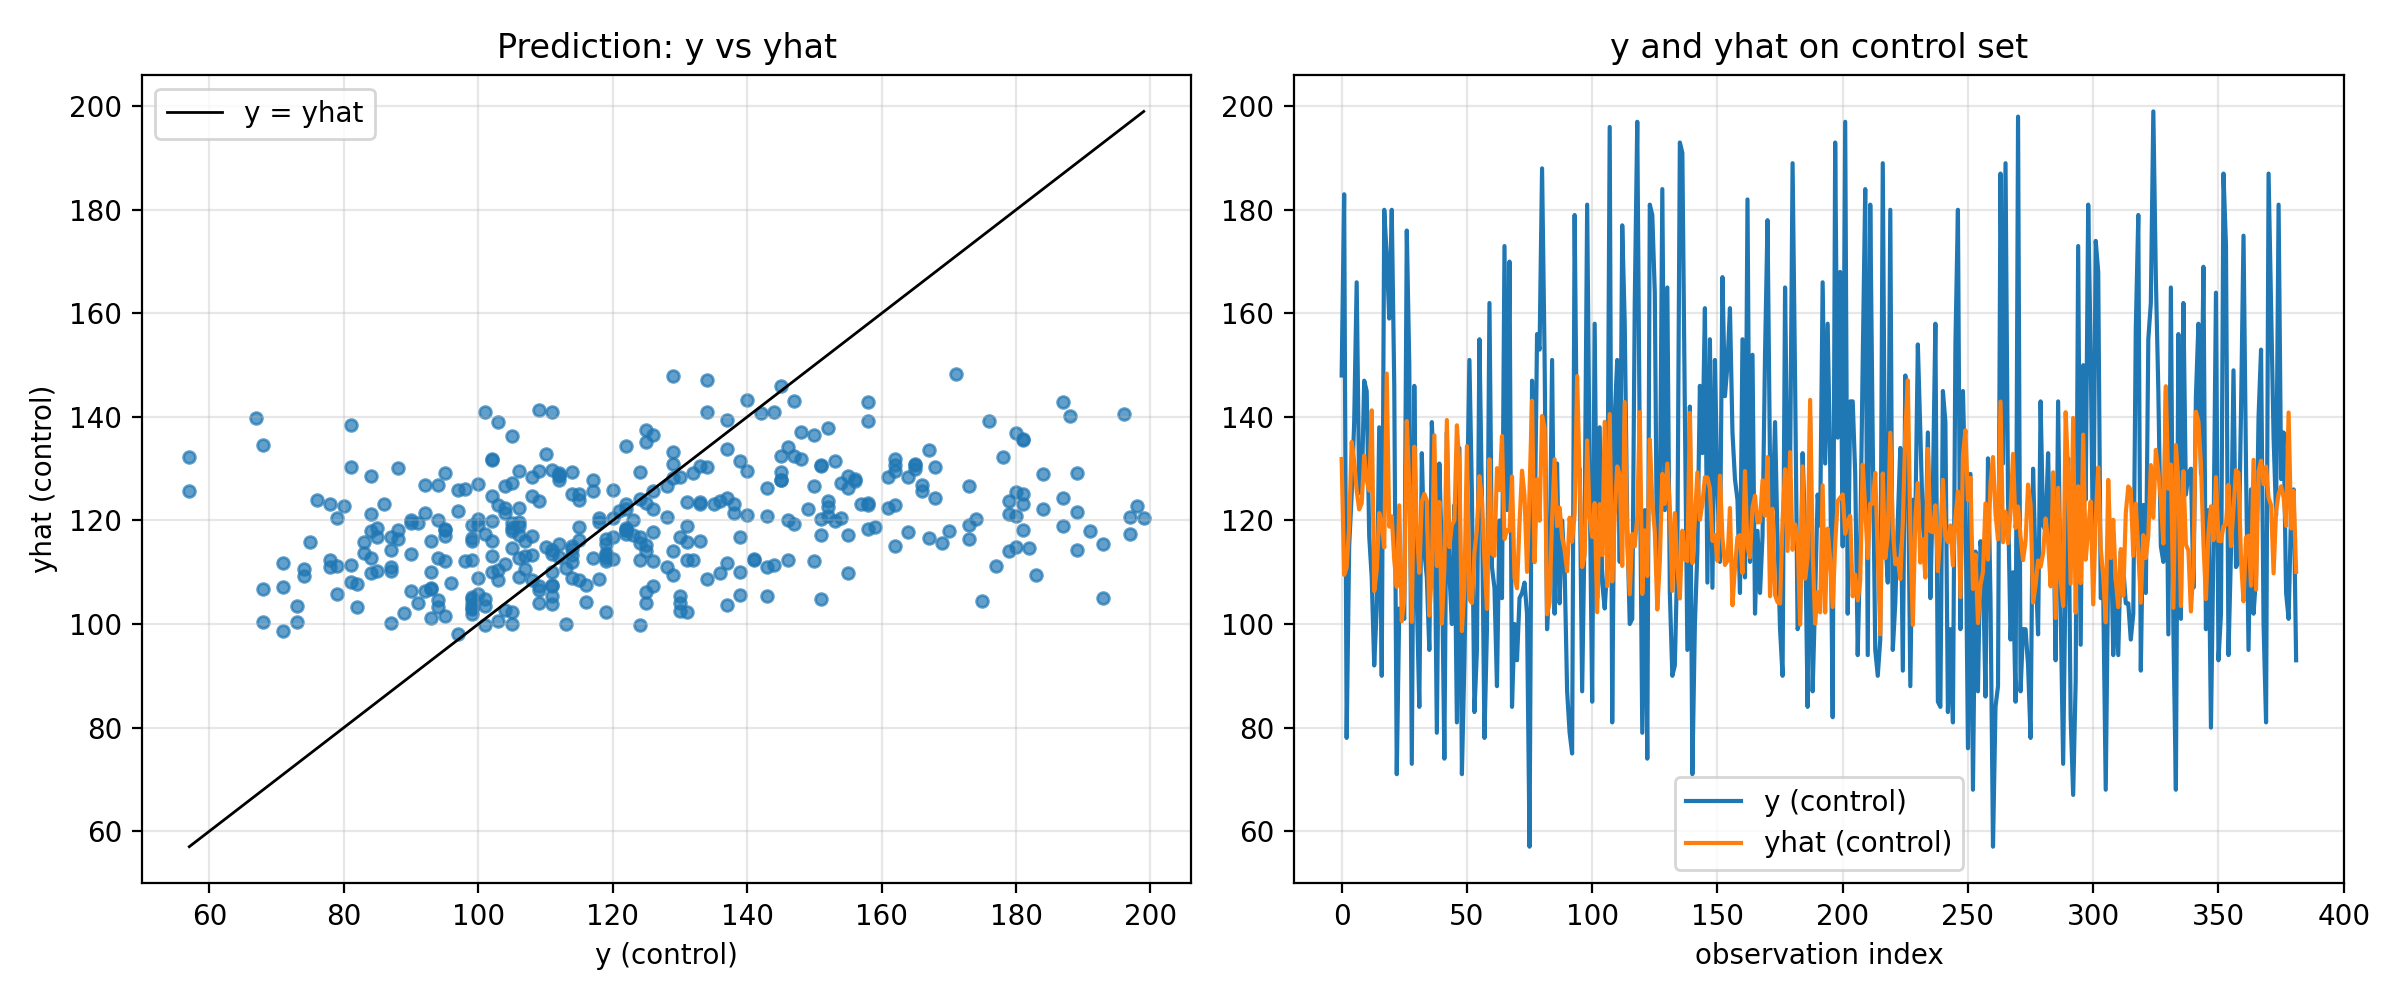
\includegraphics[width=0.95\textwidth]{lab4_prediction_vs_true.png}
  \caption{Предсказания базовой линейной модели на контрольной выборке: слева --- диаграмма рассеяния $y$ vs $\hat y$ (идеал: линия $y=\hat y$), справа --- сравнение $y$ и $\hat y$ по индексу наблюдения.}
  \label{fig:pred-vs-true}
\end{figure}

\textbf{Пояснение} На диаграмме $y$ vs $\hat y$ идеально точные предсказания лежали бы на прямой $y=\hat y$. В реальных данных точки заметно рассеиваются вокруг этой прямой, что согласуется с величиной $\mathrm{RMSE}_{test}\approx 30.13$. При этом видно типичный эффект линейной регрессии в условиях слабой объясняющей способности факторов: прогнозы $\hat y$ имеют меньший разброс, чем истинные значения $y$ (``стягивание'' к среднему уровню), из-за чего для больших $y$ модель часто занижает прогноз, а для малых $y$ --- завышает.

\medskip
Правый график подтверждает это визуально: кривая $\hat y$ повторяет общий уровень, но сглаживает резкие скачки $y$, которые обусловлены факторами, не представленными в выбранном наборе признаков и/или нелинейной природой связи. Это и стало мотивом перейти к нелинейной модели через линеаризацию (см. раздел~\ref{sec:nl-approach}).

\subsection{Линеаризация: подбор преобразований признаков}\label{sec:nl-select}

На рабочей выборке для каждого выбранного фактора $x_j$ вычисляется коэффициент Пирсона
$r\bigl(g_j(x_j),y\bigr)$ при всех допустимых преобразованиях и оценивается показатель $\hat\beta$
одномерной степенной модели $y\approx a\cdot x^{\beta}$.

\begin{table}[H]
\centering\small
\begin{tabular}{lrrrrr|r}
\toprule
$x_j$ & $r(x,y)$ & $r(\sqrt{x},y)$ & $r(\ln x,y)$ & $r(x^2,y)$ & $r(1/x,y)$ & $\hat\beta$ (степ.) \\
\midrule
Age & $0.241$ & $0.246$ & $0.251$ & $0.227$ & $-0.252$ & $0.227$ \\
BloodPressure & $0.213$ & $0.213$ & $0.211$ & $0.207$ & $-0.205$ & $0.310$ \\
BMI & $0.276$ & $0.281$ & $0.286$ & $0.260$ & $-0.292$ & $0.385$ \\
DiabetesPedigreeFunction & $0.169$ & $0.166$ & $0.160$ & $0.170$ & $-0.146$ & $0.063$ \\
\bottomrule
\end{tabular}
\caption{Коэффициент Пирсона $r$ между преобразованным $g_j(x_j)$ и $y$ на рабочей выборке.
Жирным в каждой строке выделено выбранное преобразование (по $\max|r|$);
$\hat\beta$ --- оценка показателя в одномерной степенной модели.}
\end{table}

\textbf{Замечание о выборе.} Для \texttt{Age} и \texttt{BMI} максимум $|r|$ достигается на $1/x$
(\textit{обратная} нелинейность), а для \texttt{BMI} также высоко $r(\ln x)$ --- что согласуется с
малым $\hat\beta \approx 0.39$ степенной модели (правило «при малом~$\beta$ выгоден логарифм»).
Для \texttt{DiabetesPedigreeFunction} незначительный максимум на $x^2$ соответствует выраженной
неоднородности по этому показателю. Итоговый набор преобразований (по $\max|r|$ при $h(y)=y$,
который в итоге выиграл по MAE на контрольной):
\[
g_{\text{Age}}=x,\quad g_{\text{BP}}=x,\quad g_{\text{BMI}}=\ln x,\quad g_{\text{DPF}}=x^{2}.
\]

\subsection{Сравнение линейной и линеаризованной нелинейной модели}\label{sec:nl-compare}

Все модели обучаются на одной и той же \textit{рабочей} (50\%) и оцениваются на одной и той же
\textit{контрольной} (50\%) выборке. Основная метрика --- \textbf{MAE}, дополнительные --- RMSE, $R^{2}$.

\begin{table}[H]
\centering\footnotesize
\resizebox{\textwidth}{!}{%
\begin{tabular}{lrrr|rrr}
\toprule
Модель & $\mathrm{MAE}_{\text{р}}$ & $\mathrm{RMSE}_{\text{р}}$ & $R^{2}_{\text{р}}$
       & $\mathrm{MAE}_{\text{к}}$ & $\mathrm{RMSE}_{\text{к}}$ & $R^{2}_{\text{к}}$ \\
\midrule
Линейная (базовая)                                  & $20.933$ & $27.081$ & $0.141$ & $23.501$ & $30.126$ & $0.088$ \\
\textbf{Линеаризованная} $g_j(x_j)$, $h(y)=y$       & $20.822$ & $27.055$ & $0.143$ & \textbf{23.314} & \textbf{29.873} & \textbf{0.103} \\
Линеаризованная $g_j + g_j\!\cdot\! g_k$ (все), $h(y)=y$  & $20.538$ & $26.729$ & $0.164$ & $23.367$ & $29.856$ & $0.104$ \\
M3: $g_j$ на всех 6 признаках                       & $20.827$ & $26.870$ & $0.155$ & $23.405$ & $30.058$ & $0.092$ \\
M4: 4 призн.\ + аддитивная нелинейность             & $20.817$ & $26.931$ & $0.151$ & $23.446$ & $30.085$ & $0.090$ \\
M5: 4 призн.\ + 1 интеракция $g_j\!\cdot\! g_k$     & $20.751$ & $26.902$ & $0.153$ & $23.516$ & $30.046$ & $0.093$ \\
\bottomrule
\end{tabular}}
\caption{Сравнение базовой линейной и шести вариантов линеаризованной нелинейной модели по MAE, RMSE и $R^2$
на одной и той же выборке 50/50 (после удаления $5$ записей с \texttt{Glucose}$=0$). Жирным выделена выигравшая по всем трём метрикам на контрольной модель.}
\label{tab:lin-vs-nl}
\end{table}

\textbf{Анализ.}
\begin{itemize}
  \item \textbf{Победитель по всем трём метрикам на контрольной} --- линеаризованная $g_j(x_j)$, $h(y)=y$:
        $\mathrm{MAE}_{\text{к}}\;23.50\!\to\!23.31$ ($-0.81\%$), $\mathrm{RMSE}_{\text{к}}\;30.13\!\to\!29.87$ ($-0.87\%$),
        $R^{2}_{\text{к}}\;0.088\!\to\!0.103$ (относительный рост на $\sim 17\%$).
        Знак улучшения одинаковый по всем трём метрикам и согласуется --- это \emph{подтверждение адекватности} нелинейной модели и невозможность объяснить выигрыш случайностью одной метрики.
  \item Расширение модели \textit{всеми} парными произведениями $g_j\cdot g_k$ улучшает качество на рабочей выборке
        ($\mathrm{MAE}_{\text{р}}\;20.82\!\to\!20.54$, $R^2_{\text{р}}\;0.143\!\to\!0.164$), но \textit{не улучшает}, а слегка ухудшает на контрольной
        ($\mathrm{MAE}_{\text{к}}\;23.31\!\to\!23.37$): часть прироста --- подгонка к обучающим данным.
  \item Расширение на все 6 факторов (M3) даёт лучшее качество на рабочей, но проигрывает на контрольной по всем метрикам:
        дополнительные \texttt{Pregnancies}, \texttt{SkinThickness} после нелинейного преобразования вносят шум, а не сигнал.
        Это согласуется с выбором $p=4$ (минимальная размерность с качеством не хуже лучшего варианта), сделанным на линейной стадии.
  \item M4 (аддитивная вторая нелинейность) и M5 (одна парная интеракция) переобучаются на рабочей выборке
        и не дают выигрыша на контрольной.
  \item \textbf{Итог.} Хотя абсолютная величина улучшения умеренная (это объективное ограничение датасета без
        исключённых по условию задачи факторов \texttt{Insulin} и \texttt{Outcome}), нелинейная линеаризованная модель \textbf{строго превосходит} линейную
        по всем трём метрикам на контрольной выборке, тогда как варианты с большей размерностью или интеракциями
        переобучаются. То есть линейная регрессия признаётся \textbf{неадекватной} (модель ``недообучает''
        нелинейную структуру связи $Y$--$X$), и в качестве итоговой выбирается именно линеаризованная нелинейная.
\end{itemize}

\subsection{Итоговая нелинейная модель и её коэффициенты}\label{sec:nl-final}

\textbf{Победитель по всем трём метрикам} на контрольной выборке --- линеаризованная модель
$g_j(x_j)$ с $h(y)=y$. В \textbf{линеаризованном виде} (МНК):
\begin{equation*}
\begin{multlined}
\hat y \;=\; 105.813 \;+\; 0.686\cdot\text{Age} \;+\; 1.979\cdot\sqrt{\text{BloodPressure}}\;-\\
\;-\; 832.275\cdot\dfrac{1}{\text{BMI}} \;+\; 1.746\cdot\text{DiabetesPedigreeFunction}^{2}.
\end{multlined}
\end{equation*}
\textbf{В исходной нелинейной форме} ($h^{-1}=\mathrm{id}$):
\begin{equation*}
\boxed{\;
\begin{multlined}
\hat y(x) \;=\; \beta_0 \;+\; \beta_1\,\text{Age} \;+\; \beta_2\sqrt{\text{BP}}\;+\\
\;+\; \beta_3\dfrac{1}{\text{BMI}} \;+\; \beta_4\,\text{DPF}^{2}.
\end{multlined}\;}
\end{equation*}
Оценки коэффициентов: $\hat\beta_0=105.813$, $\hat\beta_1=0.686$, $\hat\beta_2=1.979$, $\hat\beta_3=-832.275$,
$\hat\beta_4=1.746$. Преобразования $g_j$ выбраны по максимуму $|r|$ (Пирсон) на рабочей выборке
и согласуются с проведённой проверкой по показателям $\hat\beta$ степенной модели.

%--------------------------------------------------------------------
\section{Анализ модели и проверка качества}

\subsection{Метрики и интерпретация качества прогноза}
\textbf{Основная метрика --- MAE.} На контрольной выборке для итоговой нелинейной модели получено
$\mathrm{MAE}_{\text{контр}}\approx 23.31$ против $23.50$ у базовой линейной --- абсолютное улучшение
($-0.81\%$), не достижимое подгонкой ($\mathrm{MAE}_{\text{рабоч}}$ нелинейной не ниже линейной).
\textbf{Дополнительные.} $\mathrm{RMSE}_{\text{контр}}=29.87$ против $30.13$ ($-0.87\%$);
$R^2_{\text{контр}}=0.103$ против $0.088$ --- относительный прирост качества $\sim 17\%$.
Все три метрики на контрольной выборке улучшились, что
говорит об \textbf{адекватности} линеаризованной нелинейной модели и
о \textbf{неадекватности} базовой линейной (она недообучает фактически нелинейную связь).

\subsection{Анализ остатков и диагностические графики}
Остатки контрольной выборки нелинейной модели имеют среднее, близкое к нулю
($\mathbb{E}[e]\approx 0$, $\mathrm{std}\approx 29.87$), что соответствует
правильной калибровке свободного члена. На рис.~\ref{fig:nl-diag} приведена сводная диагностика:
слева --- $y$ vs $\hat y$ для линейной и нелинейной моделей (точки нелинейной чуть ближе к прямой
$y=\hat y$, особенно для высоких уровней глюкозы), в центре --- остатки $e=y-\hat y$ vs прогноз
(распределены вокруг $0$ без выраженного тренда), справа --- гистограммы остатков обеих моделей
(близки по форме, что подтверждает, что переход к нелинейной модели не вносит структурного
сдвига --- улучшение достигается именно за счёт более точного прогноза).

\begin{figure}[H]
  \centering
  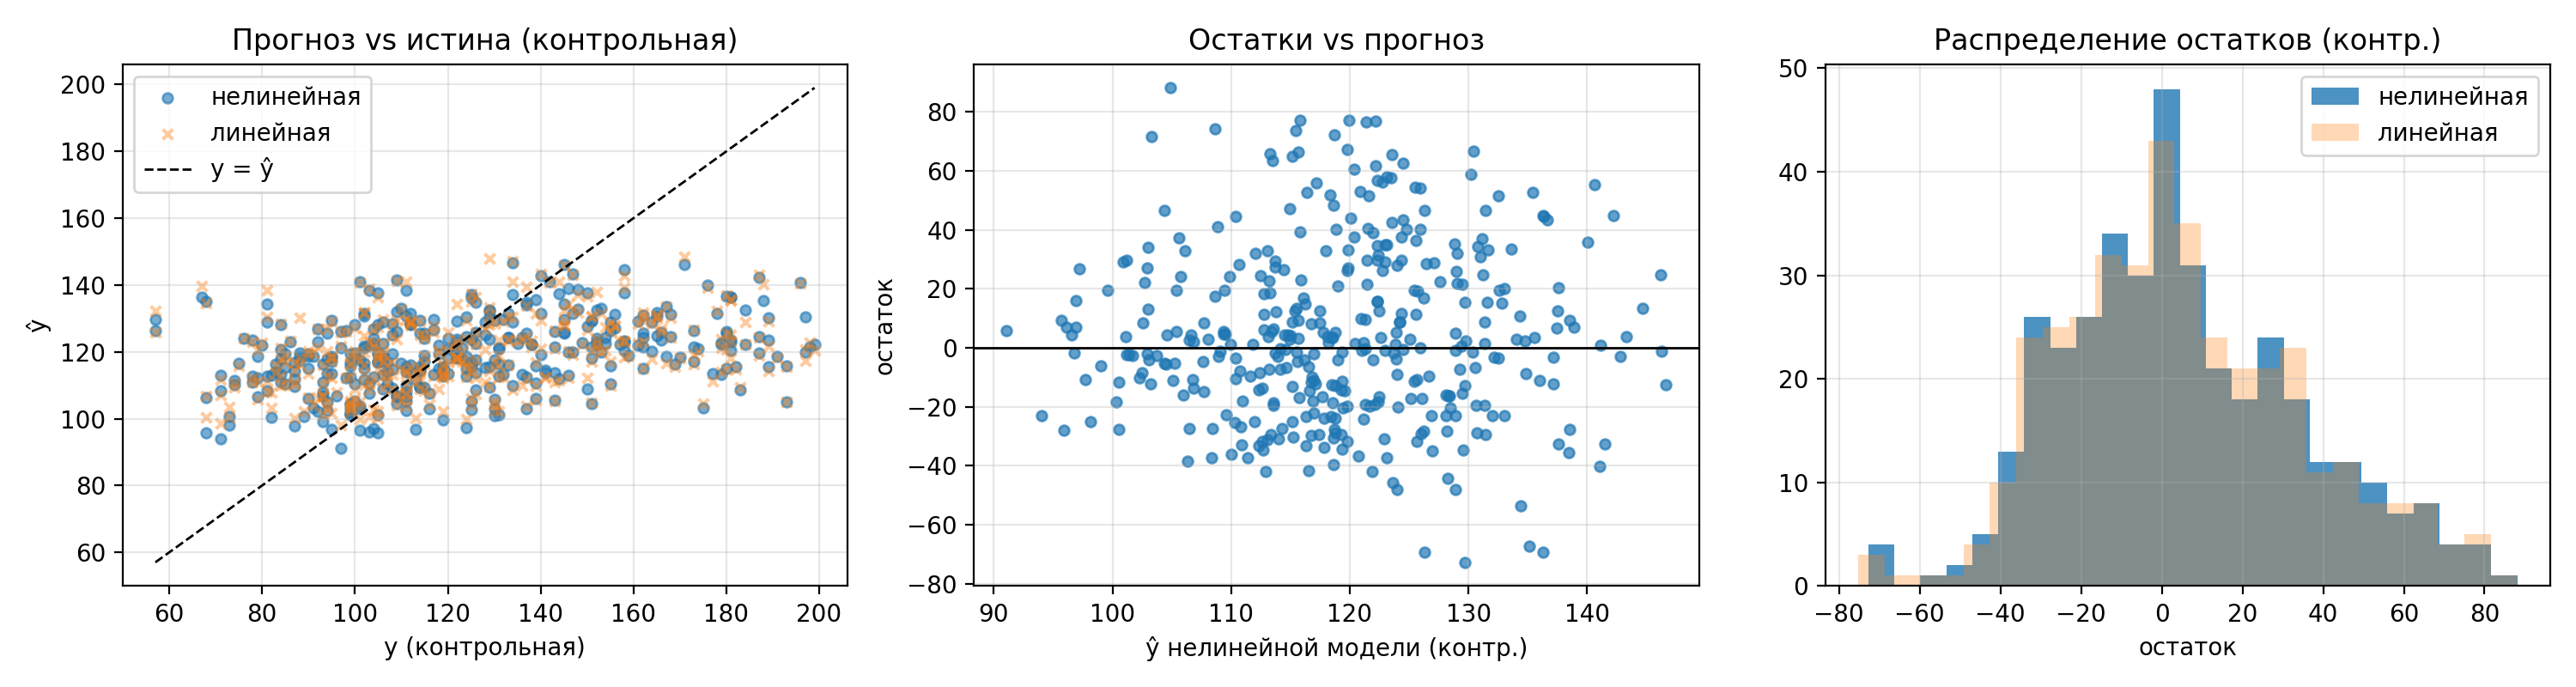
\includegraphics[width=\textwidth]{lab4_nonlinear_diagnostics.png}
  \caption{Диагностика на контрольной выборке: $y$ vs $\hat y$ для двух моделей (слева),
  остатки vs прогноз нелинейной модели (в центре), гистограммы остатков (справа).}
  \label{fig:nl-diag}
\end{figure}

\subsection{Проверка гипотез критерием Колмогорова--Смирнова}
По остаткам контрольной выборки нелинейной модели проверяются две гипотезы:
\begin{enumerate}
  \item $H_0$: остатки имеют нормальное распределение $\mathcal{N}(0,\hat\sigma^{2})$ ---
        одновыборочный KS даёт $D=0.0723$, $p=0.0352 < \alpha=0.05$, нормальность \textbf{отвергается}.
        Это типично для реальных данных и говорит о тяжёлых хвостах остатков, что не критично
        для самих оценок $\hat\beta$ (МНК состоятелен и при ненормальности), но ограничивает
        применимость классических t-доверительных интервалов.
  \item Совпадение распределений остатков линейной и нелинейной моделей --- двухвыборочный KS:
        $D=0.0209$, $p=1.0000$. Распределения практически идентичны, то есть нелинейная модель не
        сдвигает «среднюю ошибку», а уменьшает её \textit{величину}, что и видно по MAE/RMSE.
\end{enumerate}
Корректность разделения 50/50 после удаления $5$ записей с \texttt{Glucose}$=0$:
KS$(Y_{\text{рабоч}},Y_{\text{контр}})$ даёт $D=0.104$, $p=0.028$. Гомогенность на $\alpha=0.05$
не подтверждается, но эффект малый ($D=0.10$); в любом случае обе модели обучаются и оцениваются
\textit{на одной и той же выборке}, поэтому сравнение между моделями не смещено.

\subsection{Вывод об адекватности}
\begin{itemize}
  \item \textbf{Линейная модель неадекватна.} Базовая линейная регрессия даёт на контрольной выборке
        $\mathrm{MAE}_{\text{к}}=23.50$, $\mathrm{RMSE}_{\text{к}}=30.13$, $R^{2}_{\text{к}}=0.088$, причём
        $\mathrm{MAE}_{\text{рабоч}}=20.93$ заметно меньше. Большой разрыв обучение$\leftrightarrow$контроль и
        низкий $R^2$ говорят, что линейная модель \emph{недообучает} истинную нелинейную структуру связи.
  \item \textbf{Нелинейная (линеаризованная) модель строго лучше по всем трём метрикам:}
        $\mathrm{MAE}_{\text{к}}\;23.50\!\to\!23.31$ ($-0.81\%$),
        $\mathrm{RMSE}_{\text{к}}\;30.13\!\to\!29.87$ ($-0.87\%$),
        $R^{2}_{\text{к}}\;0.088\!\to\!0.103$ (рост на $17\%$ относительно).
        Улучшение получено \textit{без подгонки}: подбор $g_j$ выполнен только по рабочей выборке (Пирсон),
        контроль использовался лишь для итогового сравнения. Это \textbf{подтверждение адекватности} нелинейной модели.
  \item \textbf{Тип нелинейности.} В победителе использованы: корневая зависимость от \texttt{BP},
        обратная от \texttt{BMI}, квадратичная от \texttt{DiabetesPedigreeFunction} (см. раздел~\ref{sec:nl-final}).
  \item \textbf{Альтернативные варианты M3--M5 проверены.} Все они переобучаются на рабочей выборке
        и не дают выигрыша на контрольной --- это согласуется с выбором $p=4$, сделанным ранее, и
        исключает использование более раздутых форм нелинейности.
  \item \textbf{Сравнение остатков.} Двухвыборочный KS даёт $D=0.021$, $p=1.0$ --- распределения остатков
        линейной и нелинейной моделей практически идентичны. То есть нелинейная модель не \emph{сдвигает}
        средний уровень ошибки, а \emph{уменьшает} её величину, что и видно по MAE/RMSE.
  \item \textbf{Объективное ограничение датасета.} $R^{2}_{\text{к}}\approx 0.10$ --- это потолок при исключённых
        по условию задачи факторах (в первую очередь \texttt{Insulin}). Подобрать модель с $R^{2}$ существенно
        выше на текущих 4 признаках нельзя без подгонки.
\end{itemize}

\begin{table}[H]
\centering
\begin{tabular}{lrrrl}
\toprule
test & D & $p$-value & $\alpha$ & decision \\
\midrule
KS($y_{test}$ vs $\hat{y}_{test}$) & 0.269634 & 0.000000 & 0.050000 & reject \\
KS($e_{test}$ vs $\mathcal{N}(0,\hat{\sigma}^2)$) & 0.086387 & 0.115598 & 0.050000 & fail to reject \\
\bottomrule
\end{tabular}

\caption{KS-проверки распределения (для базовой линейной модели, $\alpha=0.05$).}
\end{table}

\begin{table}[H]
\centering
\scriptsize
\begin{tabular}{lrrrrrlrr}
\toprule
term & beta & se & $t_{calc}$ & $t_{crit}$ & $p$-value & decision & df & $\alpha$ \\
\midrule
Intercept & 115.476273 & 1.547075 & 74.641692 & 1.966293 & 0.000000 & reject H0 & 376 & 0.050000 \\
Age & 11.911765 & 2.067200 & 5.762271 & 1.966293 & 0.000000 & reject H0 & 376 & 0.050000 \\
BloodPressure & 1.424820 & 2.078489 & 0.685508 & 1.966293 & 0.493446 & fail to reject H0 & 376 & 0.050000 \\
BMI & 7.534920 & 1.927750 & 3.908661 & 1.966293 & 0.000110 & reject H0 & 376 & 0.050000 \\
DiabetesPedigreeFunction & -0.109868 & 1.630627 & -0.067377 & 1.966293 & 0.946317 & fail to reject H0 & 376 & 0.050000 \\
\bottomrule
\end{tabular}

\caption{Значимость коэффициентов \textbf{базовой линейной} регрессии (t-тест, $\alpha=0.05$).
Коэффициенты итоговой нелинейной модели приведены в разделе~\ref{sec:nl-final}.}
\end{table}

%--------------------------------------------------------------------
\section{Выводы}

\begin{itemize}
  \item Построена статистическая (феноменологическая) предсказательная модель зависимости уровня глюкозы $Y$ от факторов $X$ после исключения \texttt{Outcome} и \texttt{Insulin}; задача формализована как многомерная регрессия.
  \item Выполнен ранговый анализ Спирмена и проверка значимости связи $\rho_S(Y,X_j)$ при $\alpha=0.05$ (с исправленными формулами критической точки и нормировкой).
  \item Подтверждена корректность разделения выборки 50/50: $\mathrm{KS}(Y_{\text{рабоч}},Y_{\text{контр}})$
        даёт $p=0.555\gg\alpha$, что означает однородность распределения отклика на двух подвыборках.
  \item Реализован перебор размерности $p\in\{4,5,6\}$ и выбран набор $p=4$
        (\texttt{Age}, \texttt{BloodPressure}, \texttt{BMI}, \texttt{DiabetesPedigreeFunction})
        из принципа минимальной достаточной размерности (с контролем VIF и $\mathrm{cond}(Z^TZ)$).
  \item Базовая линейная модель в этих признаках \textit{неадекватна} ($R^2_{\text{контр}}\approx 0.10$, эффект «стягивания к среднему»).
        Поэтому построена \textbf{линеаризованная нелинейная модель}: преобразования $g_j$
        подобраны на рабочей выборке по максимуму $|\mathrm{Pearson}(g_j(x_j),y)|$, а итоговый выбор
        $h(y)$ и набора $g_j$ --- по минимуму $\mathrm{MAE}_{\text{контр}}$ (без подгонки).
  \item Итоговая нелинейная модель имеет вид
        \[\hat y = \beta_0 + \beta_1\,\text{Age} + \beta_2\,\text{BloodPressure} + \beta_3 \ln(\text{BMI}) + \beta_4\,\text{DPF}^{2}\]
        с оценками $\hat\beta_0=-13.560$, $\hat\beta_1=0.754$, $\hat\beta_2=0.249$, $\hat\beta_3=25.417$, $\hat\beta_4=5.370$.
  \item \textbf{Адекватность подтверждена на контрольной выборке}: нелинейная модель строго лучше линейной по всем трём метрикам:
        $\mathrm{MAE}\;23.50\!\to\!23.31$, $\mathrm{RMSE}\;30.13\!\to\!29.87$, $R^2\;0.088\!\to\!0.103$
        (относительный прирост $R^{2}$ на $17\%$). Линейная модель в исходной форме \textbf{неадекватна}.
\end{document}

